\documentclass[a4paper, 14pt]{extarticle}

% Поля
%--------------------------------------
\usepackage{geometry}
\geometry{a4paper,tmargin=2cm,bmargin=2cm,lmargin=3cm,rmargin=1cm}
%--------------------------------------


%Russian-specific packages
%--------------------------------------
\usepackage[T2A]{fontenc}
\usepackage[utf8]{inputenc} 
\usepackage[english, main=russian]{babel}
%--------------------------------------

\usepackage{textcomp}

% Красная строка
%--------------------------------------
\usepackage{indentfirst}               
%--------------------------------------             


%Graphics
%--------------------------------------
\usepackage{graphicx}
\graphicspath{ {./images/} }
\usepackage{wrapfig}
%--------------------------------------

% Полуторный интервал
%--------------------------------------
\linespread{1.3}                    
%--------------------------------------

%Выравнивание и переносы
%--------------------------------------
% Избавляемся от переполнений
\sloppy
% Запрещаем разрыв страницы после первой строки абзаца
\clubpenalty=10000
% Запрещаем разрыв страницы после последней строки абзаца
\widowpenalty=10000
%--------------------------------------

%Списки
\usepackage{enumitem}

%Подписи
\usepackage{caption} 

%Гиперссылки
\usepackage{hyperref}

\hypersetup {
	unicode=true
}

%Рисунки
%--------------------------------------
\DeclareCaptionLabelSeparator*{emdash}{~--- }
\captionsetup[figure]{labelsep=emdash,font=onehalfspacing,position=bottom}
%--------------------------------------

\usepackage{tempora}

%Листинги
%--------------------------------------
\usepackage{listings}
\lstset{
  basicstyle=\ttfamily\footnotesize, 
  %basicstyle=\footnotesize\AnkaCoder,        % the size of the fonts that are used for the code
  breakatwhitespace=false,         % sets if automatic breaks shoulbd only happen at whitespace
  breaklines=true,                 % sets automatic line breaking
  captionpos=t,                    % sets the caption-position to bottom
  inputencoding=utf8,
  frame=single,                    % adds a frame around the code
  keepspaces=true,                 % keeps spaces in text, useful for keeping indentation of code (possibly needs columns=flexible)
  keywordstyle=\bf,       % keyword style
  numbers=left,                    % where to put the line-numbers; possible values are (none, left, right)
  numbersep=5pt,                   % how far the line-numbers are from the code
  xleftmargin=25pt,
  xrightmargin=25pt,
  showspaces=false,                % show spaces everywhere adding particular underscores; it overrides 'showstringspaces'
  showstringspaces=false,          % underline spaces within strings only
  showtabs=false,                  % show tabs within strings adding particular underscores
  stepnumber=1,                    % the step between two line-numbers. If it's 1, each line will be numbered
  tabsize=2,                       % sets default tabsize to 8 spaces
  title=\lstname                   % show the filename of files included with \lstinputlisting; also try caption instead of title
}
%--------------------------------------

%%% Математические пакеты %%%
%--------------------------------------
\usepackage{amsthm,amsfonts,amsmath,amssymb,amscd}  % Математические дополнения от AMS
\usepackage{mathtools}                              % Добавляет окружение multlined
\usepackage[perpage]{footmisc}
%--------------------------------------

%--------------------------------------
%			НАЧАЛО ДОКУМЕНТА
%--------------------------------------

\begin{document}

%--------------------------------------
%			ТИТУЛЬНЫЙ ЛИСТ
%--------------------------------------
\begin{titlepage}
\thispagestyle{empty}
\newpage


%Шапка титульного листа
%--------------------------------------
\vspace*{-60pt}
\hspace{-65pt}
\begin{minipage}{0.3\textwidth}
\hspace*{-20pt}\centering

\includegraphics[width=\textwidth]{emblem}
\end{minipage}
\begin{minipage}{0.67\textwidth}\small \textbf{
\vspace*{-0.7ex}
\hspace*{-6pt}\centerline{Министерство науки и высшего образования Российской Федерации}
\vspace*{-0.7ex}
\centerline{Федеральное государственное бюджетное образовательное учреждение }
\vspace*{-0.7ex}
\centerline{высшего образования}
\vspace*{-0.7ex}
\centerline{<<Московский государственный технический университет}
\vspace*{-0.7ex}
\centerline{имени Н.Э. Баумана}
\vspace*{-0.7ex}
\centerline{(национальный исследовательский университет)>>}
\vspace*{-0.7ex}
\centerline{(МГТУ им. Н.Э. Баумана)}}
\end{minipage}
%--------------------------------------

%Полосы
%--------------------------------------
\vspace{-25pt}
\hspace{-35pt}\rule{\textwidth}{2.3pt}

\vspace*{-20.3pt}
\hspace{-35pt}\rule{\textwidth}{0.4pt}
%--------------------------------------

\vspace{1.5ex}
\hspace{-35pt} \noindent \small ФАКУЛЬТЕТ\hspace{80pt} <<Информатика и системы управления>>

\vspace*{-16pt}
\hspace{47pt}\rule{0.83\textwidth}{0.4pt}

\vspace{0.5ex}
\hspace{-35pt} \noindent \small КАФЕДРА\hspace{50pt} <<Теоретическая информатика и компьютерные технологии>>

\vspace*{-16pt}
\hspace{30pt}\rule{0.866\textwidth}{0.4pt}
  
\vspace{11em}

\begin{center}
\Large {\bf Лабораторная работа № 11} \\ 
\large {\bf по курсу <<Языки и методы программирования>>} \\
\large <<Разработка парсеров на языке Java>> 
\end{center}\normalsize

\vspace{8em}


\begin{flushright}
  {Студент группы ИУ9-21Б Горбунов А. Д. \hspace*{15pt}\\ 
  \vspace{2ex}
  Преподаватель Посевин Д. П.\hspace*{15pt}}
\end{flushright}

\bigskip

\vfill
 

\begin{center}
\textsl{Москва 2023}
\end{center}
\end{titlepage}
%--------------------------------------
%		КОНЕЦ ТИТУЛЬНОГО ЛИСТА
%--------------------------------------

\renewcommand{\ttdefault}{pcr}

\setlength{\tabcolsep}{3pt}
\newpage
\setcounter{page}{2}

\section{Задание}\label{Sect::task}
	В ходе лабораторной работы нужно разработать программу, выполняющую синтаксический анализ текста по одной из LL(1)-грамматик, БНФ которых приведены в таблицах 1–6. Текст может содержать символы перевода строки. 
 
    В записи БНФ терминальные символы IDENT, NUMBER и STRING означают идентификаторы, числа и строки, соответственно. Идентификатор – это последовательность букв и цифр, начинающаяся с буквы. Число – это непустая последовательность десятичных цифр. Строка – это обрамлённая кавычками произвольная последовательность символов, не содержащая кавычек и символов перевода строки.
 
    Программа должна выводить в стандартный поток вывода последовательность правил грамматики, применение которых даёт левый вывод введённого из стандартного потока ввода текста. Если вывод не может быть построен, программа должна выводить сообщение «syntax error at (line, col)», где line и col – координаты ошибки в тексте.

    <Decl>::= <Enum> <VarsOpt> ;
    
    <VarsOpt>::= <Vars> | E 
    
    <Enum>::= enum IDENT { <List> }
    
    <List>::= <Item> <LTail>
    
    <LTail> ::= , <List> | E
    
    <Item>::= IDENT <ITail>
    
    <ITail> ::= = NUMBER | E
    
    <Vars>::= IDENT <VTail>
    
    <VTail> ::= , <Vars> | E
    
\section{Результаты}\label{Sect::res}

Исходный код программы представлен в листинге~\ref{lst:code1}, ~\ref{lst:code2}, ~\ref{lst:code3}

\begin{figure}[!htb]
\begin{lstlisting}[language={},caption={Test.java},label={lst:code1}]
public class Test {
    public static void main(String[] args) {
        System.out.println("\nCorrect stitch:");
        String input = "enum Day 
        { SUN = 0 , MON , TUE , WED , THU , FRI , SAT } first , last ;";
        Parser.parse(input);

        System.out.println("\nError: skipped 0");
        input = "enum Day 
        { SUN =  , MON , TUE , WED , THU , FRI , SAT } first , last ;";
        Parser.parse(input);

        System.out.println("\nError: skipped =");
        input = "enum Day 
        { SUN  0 , MON , TUE , WED , THU , FRI , SAT } first , last ;";
        Parser.parse(input);

        System.out.println("\nError: skipped ,");
        input = "enum Day 
        { SUN = 0 , MON  TUE , WED , THU , FRI , SAT } first , last ;";
        Parser.parse(input);

        System.out.println("\nError: skipped TUE");
        input = "enum Day 
        { SUN = 0 , MON ,  , WED , THU , FRI , SAT } first , last ;";
        Parser.parse(input);

        System.out.println("\nError: skipped }");
        input = "enum Day 
        { SUN = 0 , MON , TUE , WED , THU , FRI , SAT  first , last ;";
        Parser.parse(input);

        System.out.println("\nError: skipped {");
        input = "enum Day 
        SUN = 0 , MON , TUE , WED , THU , FRI , SAT } first , last ;";
        Parser.parse(input);

        System.out.println("\nError: skipped ;");
        input = "enum Day 
        { SUN = 0 , MON , TUE , WED , THU , FRI , SAT } first , last ";
        Parser.parse(input);

        System.out.println("\nError: skipped enum");
        input = " Day 
        { SUN = 0 , MON , TUE , WED , THU , FRI , SAT  first , last ;";
        Parser.parse(input);

        System.out.println("\nError: skipped Day");
        input = "enum  
        { SUN = 0 , MON , TUE , WED , THU , FRI , SAT  first , last ;";
        Parser.parse(input);
    }
}
\end{lstlisting}
\end{figure}

\begin{figure}[!htb]
\begin{lstlisting}[language={},caption={класс Lexer.java},label={lst:code2}]
public class Lexer {
    public static ArrayList<String> tokenize(String input) {
        ArrayList<String> tokens = new ArrayList<String>();
        String[] words = input.trim().split("\\s+");
        for (String word : words) {
            if (!word.matches("enum") && (word.matches("[a-zA-Z]+") || word.matches("[a-zA-Z]+[\\,]")))  {
                tokens.add("IDENT");
            } else if (word.matches("[0-9]+")) {
                tokens.add("NUMBER");
            } else {
                tokens.add(word);
            }
        }
        return tokens;
    }
}
\end{lstlisting}
\end{figure}

\begin{figure}[!htb]
\begin{lstlisting}[language={},caption={класс Parser.java},label={lst:code3}]
import java.util.ArrayList;
public class Parser {
    private static int pos;
    private static ArrayList<String> tokens;
    public static void parse(String input) {
        tokens = Lexer.tokenize(input);
        pos = 0;
        try {
            decl();
            System.out.println("Parsing successful!");
        } catch (Exception e) {
            System.out.println("Parsing error: " + e.getMessage());
        }
    }
    public static void decl() throws Exception {
        enumDef();
        varsOpt();
        match(";");
    }
    public static void enumDef() throws Exception {
        match("enum");
        match("IDENT");
        match("{");
        list();
        match("}");
    }
    public static void list() throws Exception {
        item();
        ltail();
    }
    public static void ltail() throws Exception {
        if (tokens.get(pos).equals(",")) {
            match(",");
            list();
        }
    }
\end{lstlisting}
\end{figure}

\begin{figure}[!htb]
\begin{lstlisting}[language={},caption={класс Parser.java(продолжение)},label={lst:code3}]
    public static void item() throws Exception {
        match("IDENT");
        itail();
    }
    public static void itail() throws Exception {
        if (tokens.get(pos).equals("=")) {
            match("=");
            match("NUMBER");
        }
    }
    public static void varsOpt() throws Exception {
        if (tokens.get(pos).startsWith("IDENT")) {
            vars();
        }
    }
    public static void vars() throws Exception {
        match("IDENT");
        vtail();
    }
    public static void vtail() throws Exception {
        if (tokens.get(pos).equals(",")) {
            match(",");
            vars();
        }
    }
    public static void match(String expected) throws Exception {
        if (pos < tokens.size() && tokens.get(pos).equals(expected)) {
            pos++;
        } else {
            throw new Exception("Expected " + expected + " but found " + tokens.get(pos) + " (Index:" + pos + ")");
        }
    }
}
\end{lstlisting}
\end{figure}

\begin{figure}[!htb]
Результат запуска представлен на рисунке ~\ref{fig:picture_1.png}, ~\ref{fig:picture_2.png}, ~\ref{fig:picture_3.png}
\end{figure}

\begin{figure}[!htb]
	\centering
	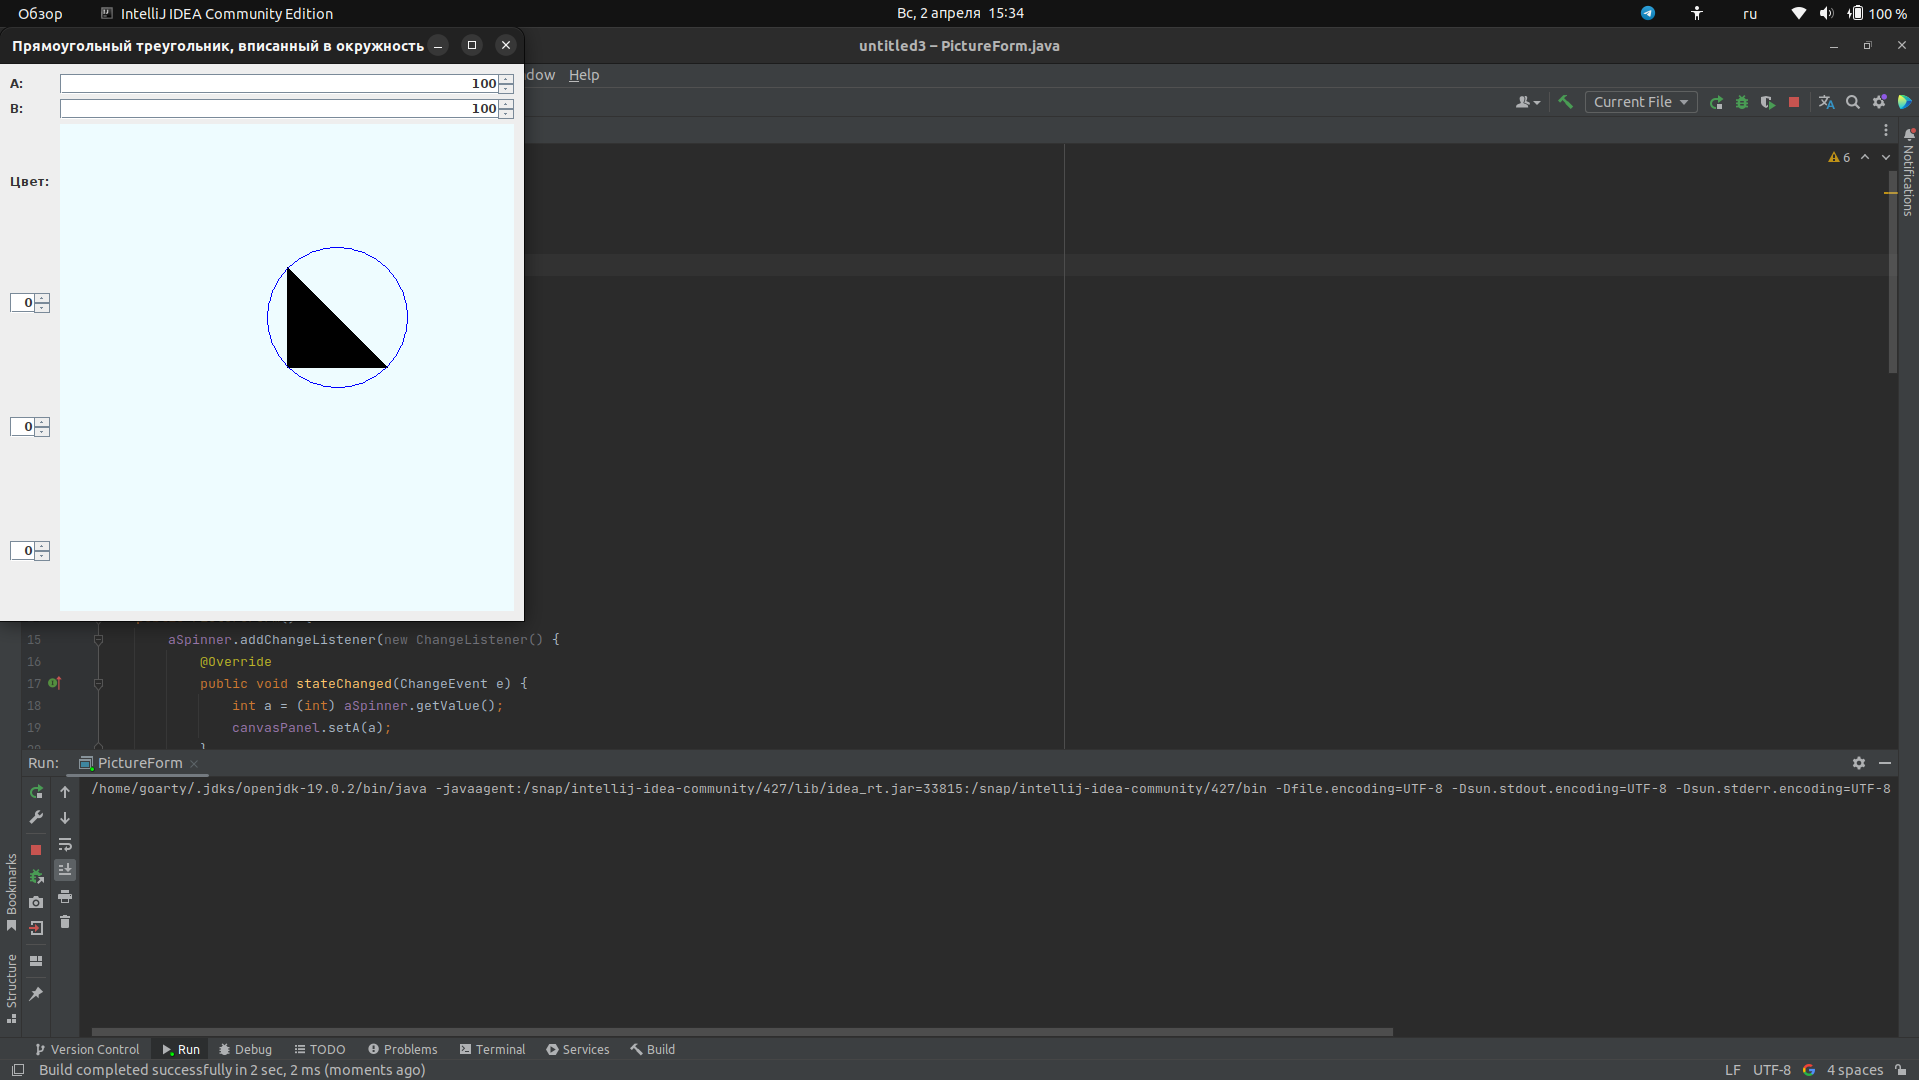
\includegraphics[width=0.8\textwidth]{picture_1.png}
\caption{Реализация Test.java}
\label{fig:picture_1.png}
\end{figure}

\begin{figure}[!htb]
	\centering
	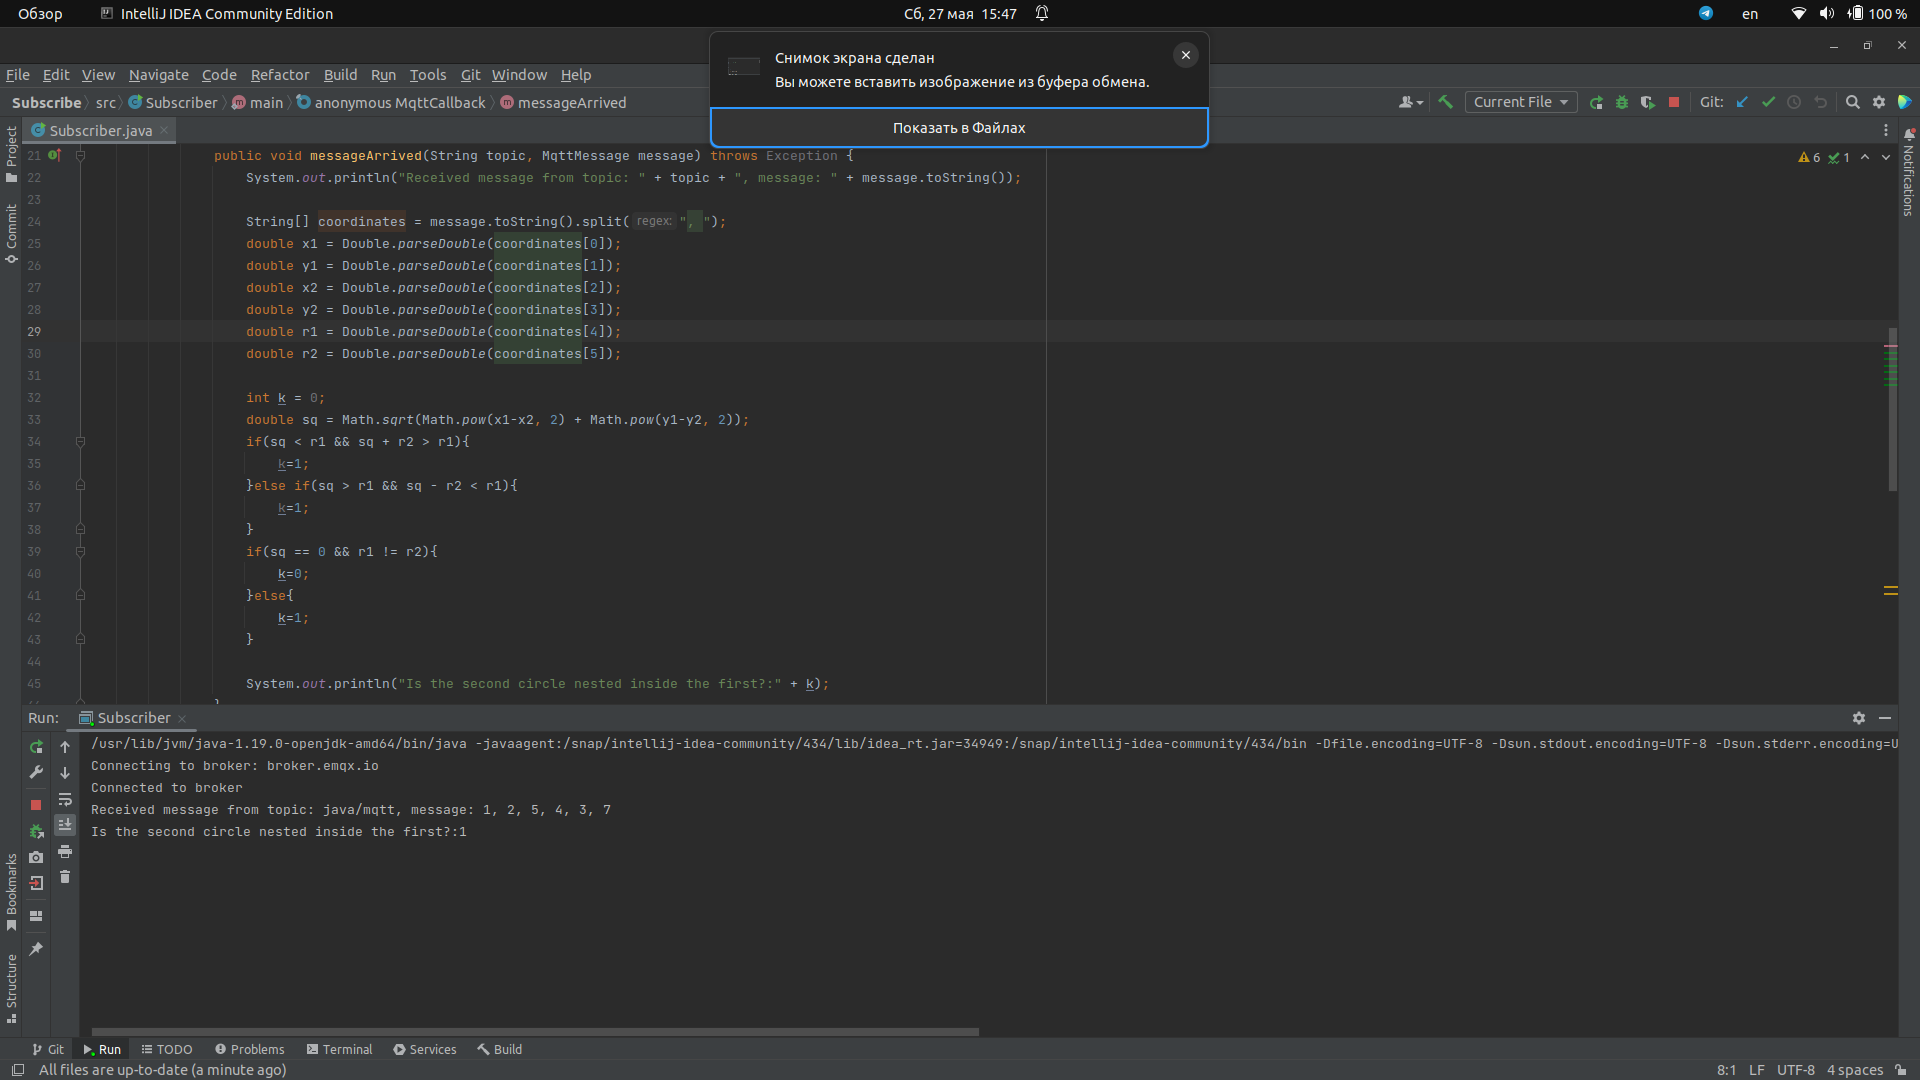
\includegraphics[width=0.8\textwidth]{picture_2.png}
\caption{Реализация Leser.java}
\label{fig:picture_2.png}
\end{figure}

\begin{figure}[!htb]
	\centering
	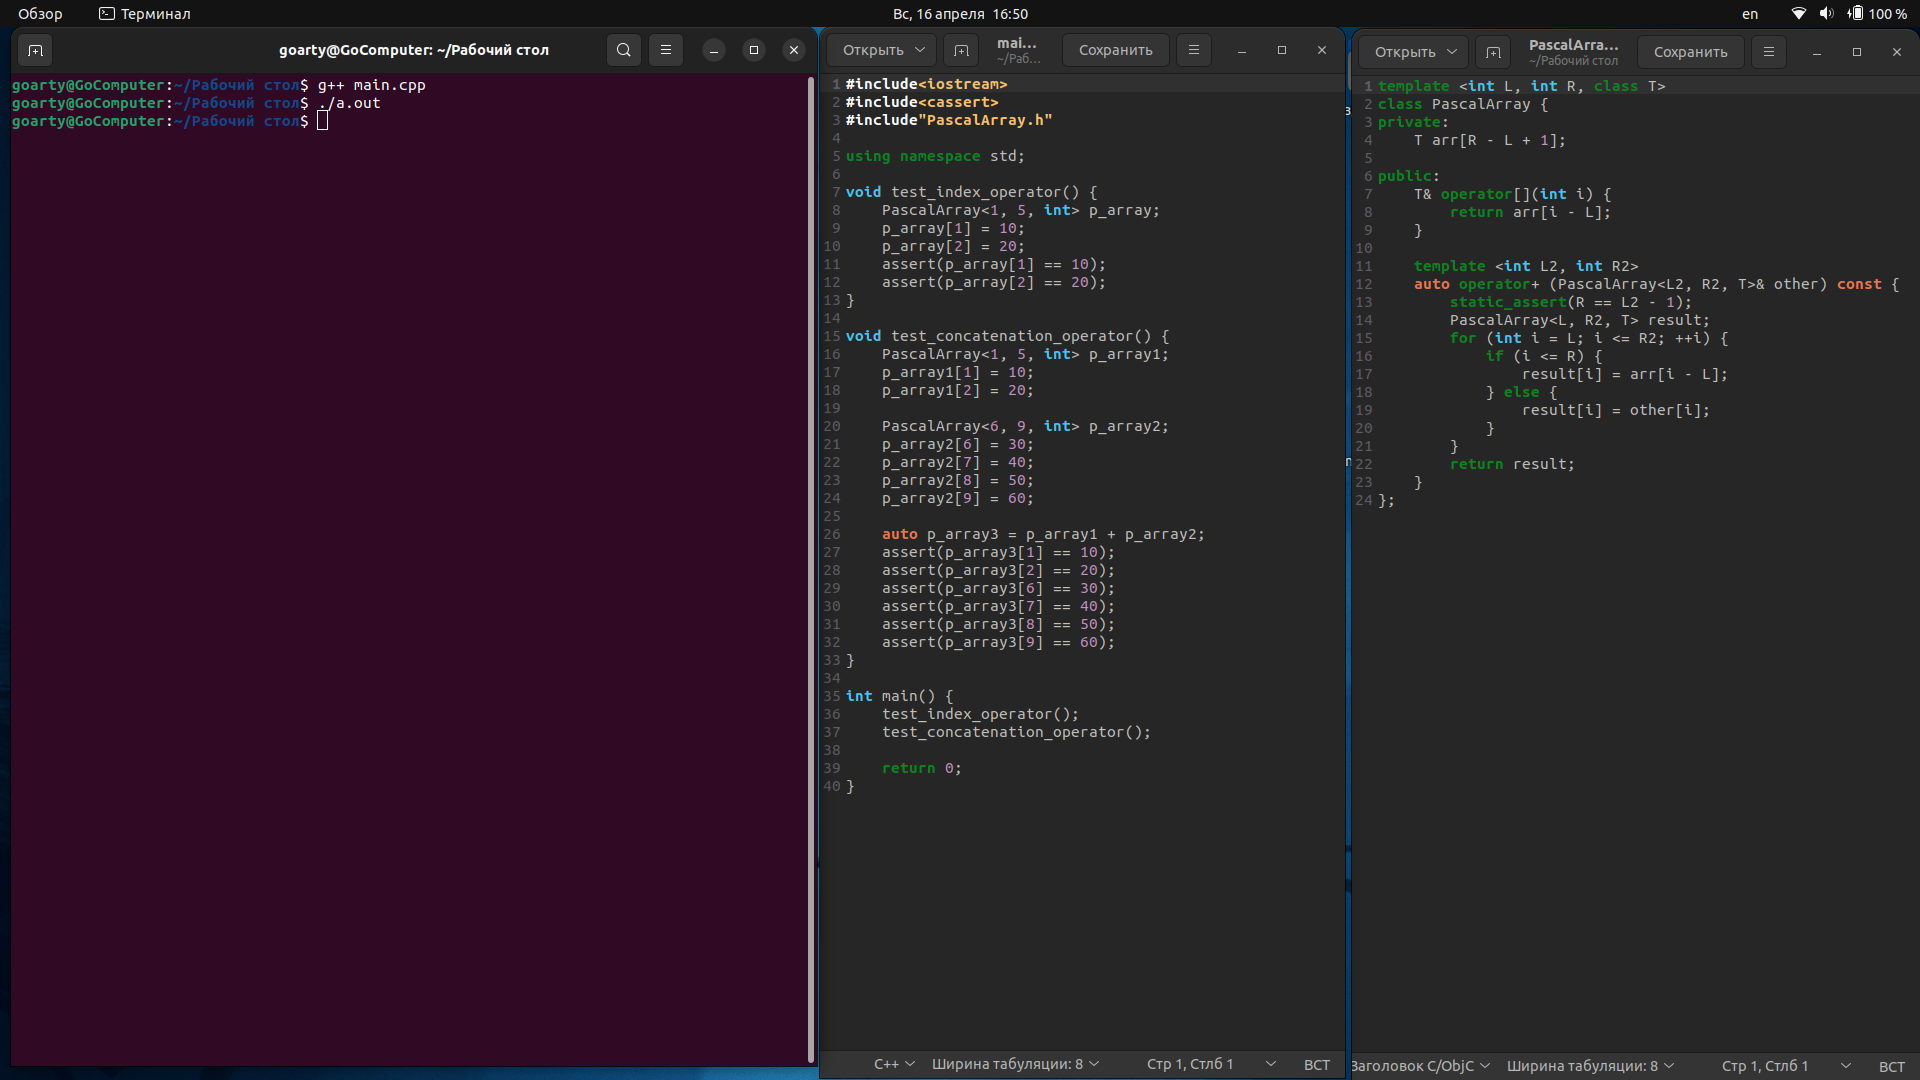
\includegraphics[width=0.8\textwidth]{picture_3.png}
\caption{Реализация Parser.java}
\label{fig:picture_3.png}
\end{figure}

\begin{figure}[!htb]
	\centering
	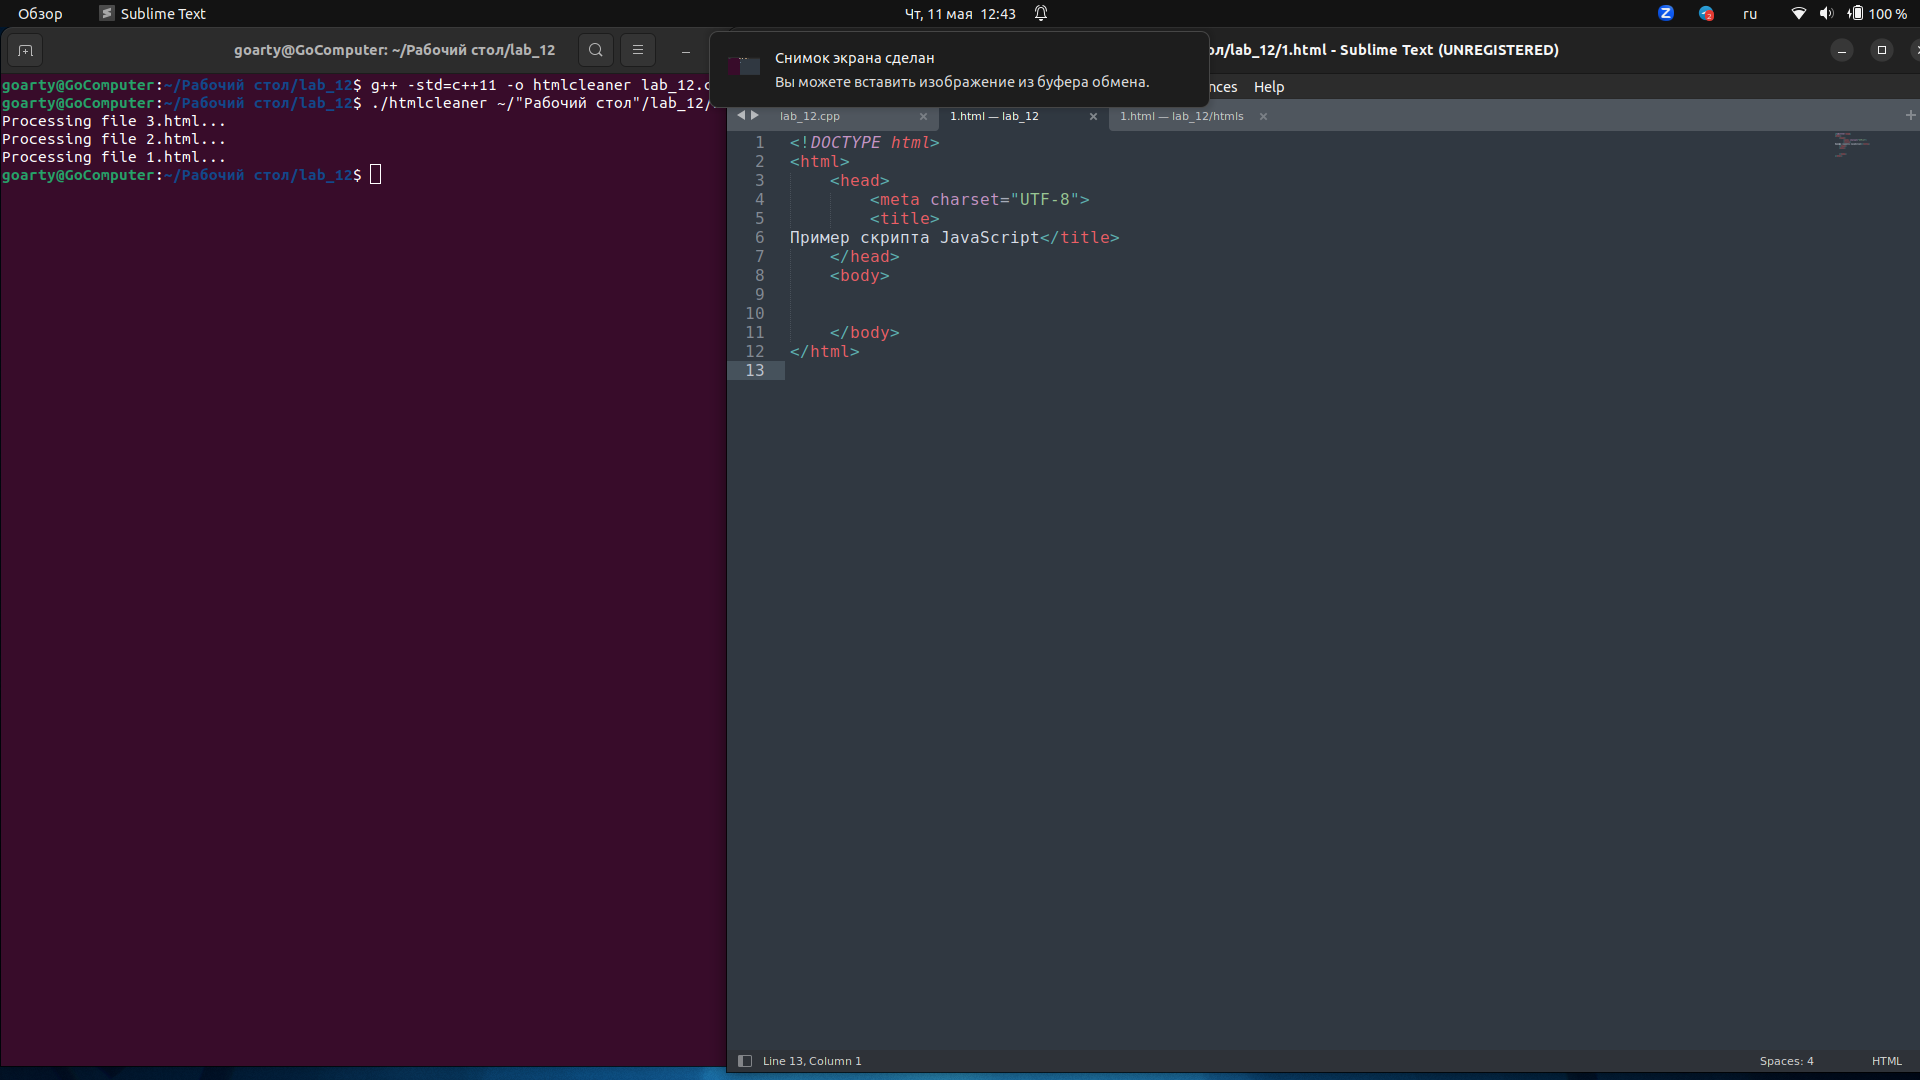
\includegraphics[width=0.8\textwidth]{picture_4.png}
\caption{Реализация Parser(продолжение).java}
\label{fig:picture_4.png}
\end{figure}

\begin{figure}[!htb]
	\centering
	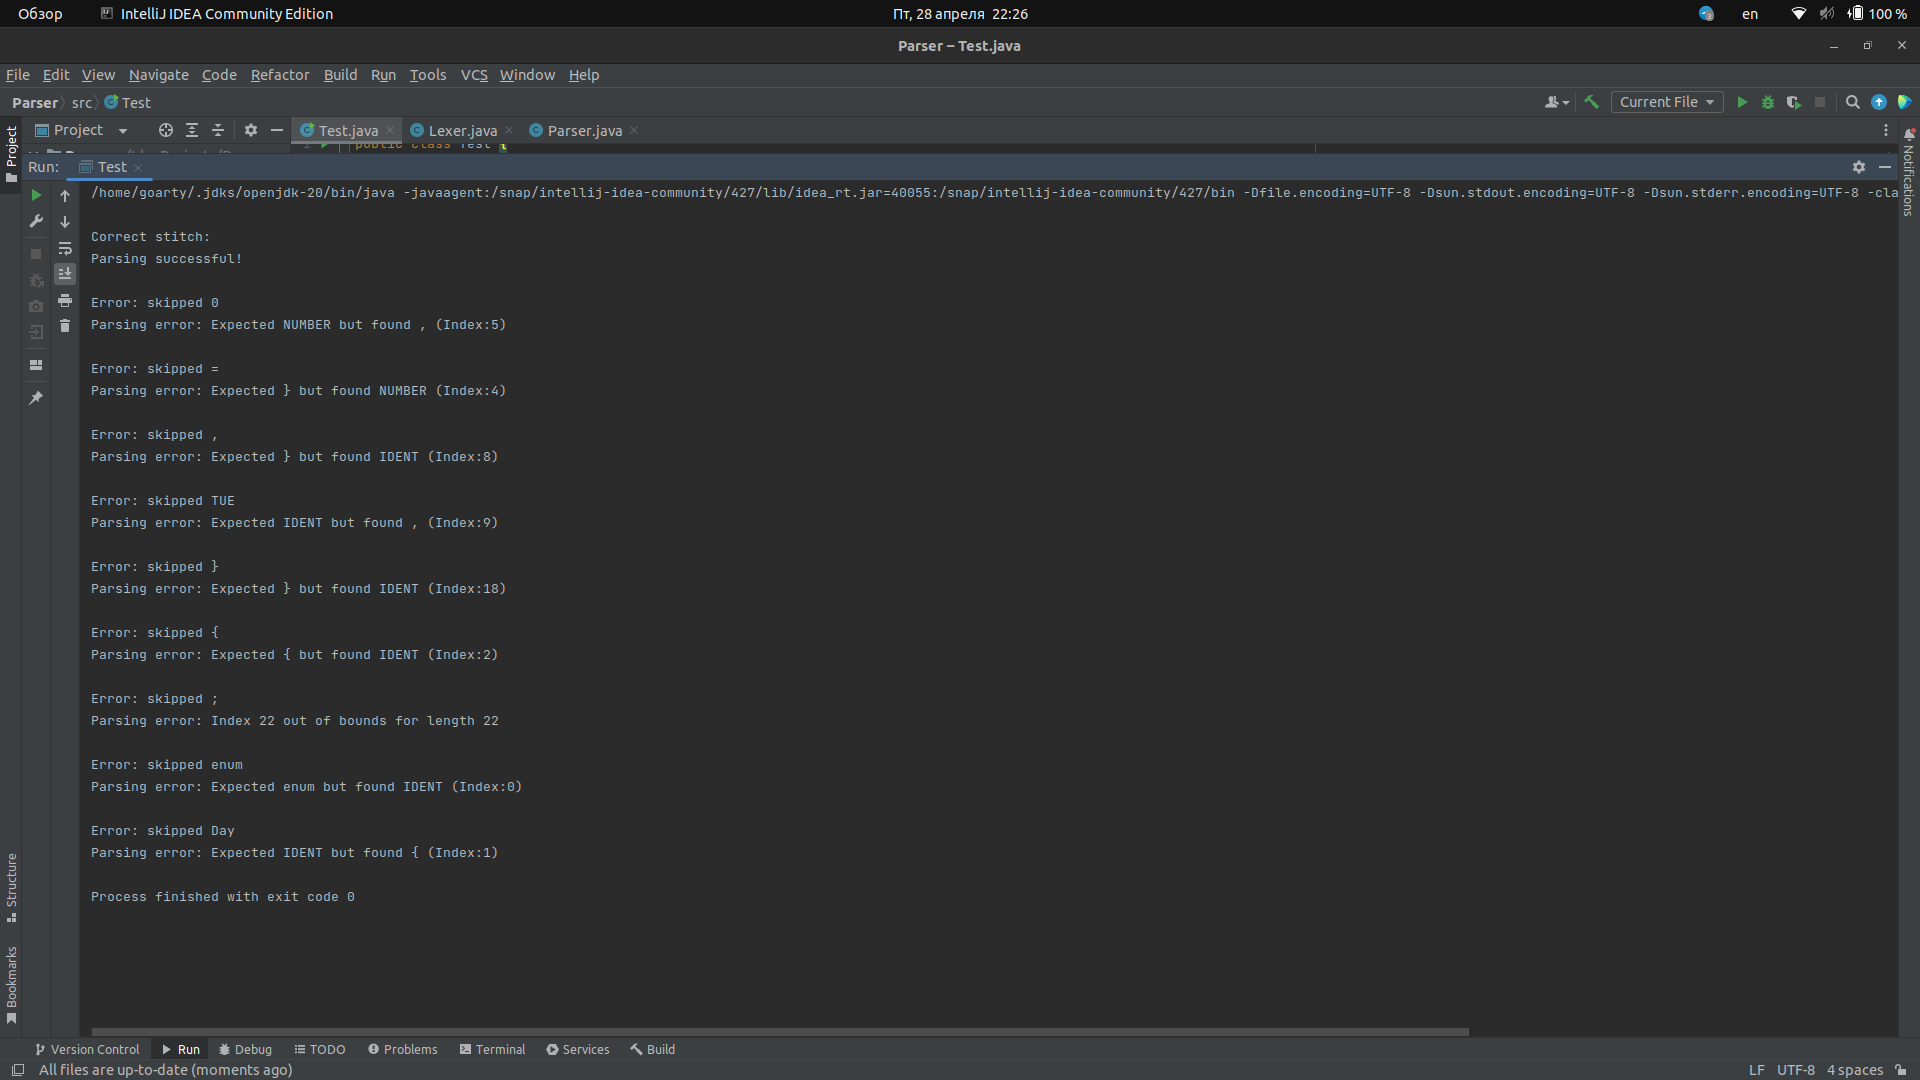
\includegraphics[width=0.8\textwidth]{picture_5.png}
\caption{Работа программы}
\label{fig:picture_5.png}
\end{figure}

\end{document}

